%%%%%%%%%%%%%%%%%%%%%%%%%%%%%%%%%%%%%%%%%
% The Legrand Orange Book
% LaTeX Template
% Version 2.1.1 (14/2/16)
%
% This template has been downloaded from:
% http://www.LaTeXTemplates.com
%
% Original author:
% Mathias Legrand (legrand.mathias@gmail.com) with modifications by:
% Vel (vel@latextemplates.com)
%
% License:
% CC BY-NC-SA 3.0 (http://creativecommons.org/licenses/by-nc-sa/3.0/)
%
% Compiling this template:
% This template uses biber for its bibliography and makeindex for its index.
% When you first open the template, compile it from the command line with the 
% commands below to make sure your LaTeX distribution is configured correctly:
%
% 1) pdflatex main
% 2) makeindex main.idx -s StyleInd.ist
% 3) biber main
% 4) pdflatex main x 2
%
% After this, when you wish to update the bibliography/index use the appropriate
% command above and make sure to compile with pdflatex several times 
% afterwards to propagate your changes to the document.
%
% This template also uses a number of packages which may need to be
% updated to the newest versions for the template to compile. It is strongly
% recommended you update your LaTeX distribution if you have any
% compilation errors.
%
% Important note:
% Chapter heading images should have a 2:1 width:height ratio,
% e.g. 920px width and 460px height.
%
%%%%%%%%%%%%%%%%%%%%%%%%%%%%%%%%%%%%%%%%%

%----------------------------------------------------------------------------------------
%	PACKAGES AND OTHER DOCUMENT CONFIGURATIONS
%----------------------------------------------------------------------------------------

\documentclass[11pt,fleqn, openany]{book} % Default font size and left-justified equations
% \usepackage{verbatim}
\usepackage{listings}

%----------------------------------------------------------------------------------------

%%%%%%%%%%%%%%%%%%%%%%%%%%%%%%%%%%%%%%%%%
% The Legrand Orange Book
% Structural Definitions File
% Version 2.0 (9/2/15)
%
% Original author:
% Mathias Legrand (legrand.mathias@gmail.com) with modifications by:
% Vel (vel@latextemplates.com)
% 
% This file has been downloaded from:
% http://www.LaTeXTemplates.com
%
% License:
% CC BY-NC-SA 3.0 (http://creativecommons.org/licenses/by-nc-sa/3.0/)
%
%%%%%%%%%%%%%%%%%%%%%%%%%%%%%%%%%%%%%%%%%

%----------------------------------------------------------------------------------------
%	VARIOUS REQUIRED PACKAGES AND CONFIGURATIONS
%----------------------------------------------------------------------------------------

\usepackage[top=3cm,bottom=3cm,left=3cm,right=3cm,headsep=10pt,a4paper]{geometry} % Page margins

\usepackage{graphicx} % Required for including pictures
\graphicspath{{Pictures/}} % Specifies the directory where pictures are stored

\usepackage{lipsum} % Inserts dummy text

\usepackage{tikz} % Required for drawing custom shapes

\usepackage[english]{babel} % English language/hyphenation

\usepackage{enumitem} % Customize lists
\setlist{nolistsep} % Reduce spacing between bullet points and numbered lists

\usepackage{booktabs} % Required for nicer horizontal rules in tables

\usepackage[dvipsnames]{xcolor} % Required for specifying colors by name
\definecolor{myWhite}{RGB}{255, 255, 255}
\definecolor{Green}{RGB}{185, 219, 125} % Define the orange color used for highlighting throughout the book

%----------------------------------------------------------------------------------------
%	FONTS
%----------------------------------------------------------------------------------------

\usepackage{avant} % Use the Avantgarde font for headings
%\usepackage{times} % Use the Times font for headings
\usepackage{mathptmx} % Use the Adobe Times Roman as the default text font together with math symbols from the Sym­bol, Chancery and Com­puter Modern fonts

\usepackage{microtype} % Slightly tweak font spacing for aesthetics
\usepackage[utf8]{inputenc} % Required for including letters with accents
\usepackage[T1]{fontenc} % Use 8-bit encoding that has 256 glyphs

\renewcommand*\rmdefault{cmbr} % COMPUTER BRIGHT PER IL TESTO
\renewcommand*\sfdefault{pag} % Imposta Avantgarde come sans-serif % AVANTGARDE PER I TITOLI

%----------------------------------------------------------------------------------------
%	BIBLIOGRAPHY AND INDEX
%----------------------------------------------------------------------------------------

\usepackage{csquotes}
\usepackage[style=alphabetic,citestyle=numeric,sorting=nyt,sortcites=true,autopunct=true,autolang=hyphen,hyperref=true,abbreviate=false,backref=true,backend=biber,defernumbers=true]{biblatex}
\addbibresource{bibliography.bib} % BibTeX bibliography file
\defbibheading{bibempty}{}

\usepackage{calc} % For simpler calculation - used for spacing the index letter headings correctly
\usepackage{makeidx} % Required to make an index
\makeindex % Tells LaTeX to create the files required for indexing

%----------------------------------------------------------------------------------------
%	MAIN TABLE OF CONTENTS
%----------------------------------------------------------------------------------------

\usepackage{titletoc} % Required for manipulating the table of contents

\contentsmargin{0cm} % Removes the default margin

% Part text styling
\titlecontents{part}[0cm]
{\addvspace{20pt}\centering\large\bfseries}
{}
{}
{}

% Chapter text styling
\titlecontents{chapter}[1.25cm] % Indentation
{\addvspace{12pt}\large\sffamily\bfseries} % Spacing and font options for chapters
{\color{Green!60}\contentslabel[\Large\thecontentslabel]{1.25cm}\color{Green}} % Chapter number
{\color{Green}}  
{\color{Green!60}\normalsize\;\titlerule*[.5pc]{.}\;\thecontentspage} % Page number

% Section text styling
\titlecontents{section}[1.25cm] % Indentation
{\addvspace{3pt}\sffamily\bfseries} % Spacing and font options for sections
{\contentslabel[\thecontentslabel]{1.25cm}} % Section number
{}
{\hfill\color{black}\thecontentspage} % Page number
[]

% Subsection text styling
\titlecontents{subsection}[1.25cm] % Indentation
{\addvspace{1pt}\sffamily\small} % Spacing and font options for subsections
{\contentslabel[\thecontentslabel]{1.25cm}} % Subsection number
{}
{\ \titlerule*[.5pc]{.}\;\thecontentspage} % Page number
[]

% List of figures
\titlecontents{figure}[0em]
{\addvspace{-5pt}\sffamily}
{\thecontentslabel\hspace*{1em}}
{}
{\ \titlerule*[.5pc]{.}\;\thecontentspage}
[]

% List of tables
\titlecontents{table}[0em]
{\addvspace{-5pt}\sffamily}
{\thecontentslabel\hspace*{1em}}
{}
{\ \titlerule*[.5pc]{.}\;\thecontentspage}
[]

%----------------------------------------------------------------------------------------
%	MINI TABLE OF CONTENTS IN PART HEADS
%----------------------------------------------------------------------------------------

% Chapter text styling
\titlecontents{lchapter}[0em] % Indenting
{\addvspace{15pt}\large\sffamily\bfseries} % Spacing and font options for chapters
{\color{Green}\contentslabel[\Large\thecontentslabel]{1.25cm}\color{Green}} % Chapter number
{}  
{\color{Green}\normalsize\sffamily\bfseries\;\titlerule*[.5pc]{.}\;\thecontentspage} % Page number

% Section text styling
\titlecontents{lsection}[0em] % Indenting
{\sffamily\small} % Spacing and font options for sections
{\contentslabel[\thecontentslabel]{1.25cm}} % Section number
{}
{}

% Subsection text styling
\titlecontents{lsubsection}[.5em] % Indentation
{\normalfont\footnotesize\sffamily} % Font settings
{}
{}
{}

%----------------------------------------------------------------------------------------
%	PAGE HEADERS
%----------------------------------------------------------------------------------------

\usepackage{fancyhdr} % Required for header and footer configuration

\pagestyle{fancy}
\renewcommand{\chaptermark}[1]{\markboth{\sffamily\normalsize\bfseries\chaptername\ \thechapter.\ #1}{}} % Chapter text font settings
\renewcommand{\sectionmark}[1]{\markright{\sffamily\normalsize\thesection\hspace{5pt}#1}{}} % Section text font settings
\fancyhf{} \fancyhead[LE,RO]{\sffamily\normalsize\thepage} % Font setting for the page number in the header
\fancyhead[LO]{\rightmark} % Print the nearest section name on the left side of odd pages
\fancyhead[RE]{\leftmark} % Print the current chapter name on the right side of even pages
\renewcommand{\headrulewidth}{0.5pt} % Width of the rule under the header
\addtolength{\headheight}{2.5pt} % Increase the spacing around the header slightly
\renewcommand{\footrulewidth}{0pt} % Removes the rule in the footer
\fancypagestyle{plain}{\fancyhead{}\renewcommand{\headrulewidth}{0pt}} % Style for when a plain pagestyle is specified

% Removes the header from odd empty pages at the end of chapters
\makeatletter
\renewcommand{\cleardoublepage}{
\clearpage\ifodd\c@page\else
\hbox{}
\vspace*{\fill}
\thispagestyle{empty}
\newpage
\fi}

%----------------------------------------------------------------------------------------
%	THEOREM STYLES
%----------------------------------------------------------------------------------------

\usepackage{amsmath,amsfonts,amssymb,amsthm} % For math equations, theorems, symbols, etc

\newcommand{\intoo}[2]{\mathopen{]}#1\,;#2\mathclose{[}}
\newcommand{\ud}{\mathop{\mathrm{{}d}}\mathopen{}}
\newcommand{\intff}[2]{\mathopen{[}#1\,;#2\mathclose{]}}
\newtheorem{notation}{Notation}[chapter]

% Boxed/framed environments
\newtheoremstyle{Greennumbox}% % Theorem style name
{0pt}% Space above
{0pt}% Space below
{\normalfont}% % Body font
{}% Indent amount
{\small\bf\sffamily\color{Green}}% % Theorem head font
{\;}% Punctuation after theorem head
{0.25em}% Space after theorem head
{\small\sffamily\color{Green}\thmname{#1}\nobreakspace\thmnumber{\@ifnotempty{#1}{}\@upn{#2}}% Theorem text (e.g. Theorem 2.1)
\thmnote{\nobreakspace\the\thm@notefont\sffamily\bfseries\color{black}---\nobreakspace#3.}} % Optional theorem note
\renewcommand{\qedsymbol}{$\blacksquare$}% Optional qed square

\newtheoremstyle{blacknumex}% Theorem style name
{5pt}% Space above
{5pt}% Space below
{\normalfont}% Body font
{} % Indent amount
{{\small\bf\sffamily\color{Green}}}% Theorem head font
{\;}% Punctuation after theorem head
{0.25em}% Space after theorem head
{\small\sffamily{\tiny\ensuremath{\blacksquare}}\nobreakspace\thmname{#1}\nobreakspace\thmnumber{\@ifnotempty{#1}{}\@upn{#2}}% Theorem text (e.g. Theorem 2.1)
\thmnote{\nobreakspace\the\thm@notefont\sffamily\bfseries---\nobreakspace#3.}}% Optional theorem note

\newtheoremstyle{blacknumbox} % Theorem style name
{0pt}% Space above
{0pt}% Space below
{\normalfont}% Body font
{}% Indent amount
{\small\bf\sffamily}% Theorem head font
{\;}% Punctuation after theorem head
{0.25em}% Space after theorem head
{\small\sffamily\thmname{#1}\nobreakspace\thmnumber{\@ifnotempty{#1}{}\@upn{#2}}% Theorem text (e.g. Theorem 2.1)
\thmnote{\nobreakspace\the\thm@notefont\sffamily\bfseries---\nobreakspace#3.}}% Optional theorem note

% Non-boxed/non-framed environments
\newtheoremstyle{Greennum}% % Theorem style name
{5pt}% Space above
{5pt}% Space below
{\normalfont}% % Body font
{}% Indent amount
{\small\bf\sffamily\color{Green}}% % Theorem head font
{\;}% Punctuation after theorem head
{0.25em}% Space after theorem head
{\small\sffamily\color{Green}\thmname{#1}\nobreakspace\thmnumber{\@ifnotempty{#1}{}\@upn{#2}}% Theorem text (e.g. Theorem 2.1)
\thmnote{\nobreakspace\the\thm@notefont\sffamily\bfseries\color{black}---\nobreakspace#3.}} % Optional theorem note
\renewcommand{\qedsymbol}{$\blacksquare$}% Optional qed square
\makeatother

% Defines the theorem text style for each type of theorem to one of the three styles above
\newcounter{dummy} 
\numberwithin{dummy}{section}
\theoremstyle{Greennumbox}
\newtheorem{theoremeT}[dummy]{Theorem}
\newtheorem{problem}{Problem}[chapter]
\newtheorem{exerciseT}{Exercise}[chapter]
\theoremstyle{blacknumex}
\newtheorem{exampleT}{\textbf{Nota Bene}}[chapter]
\theoremstyle{blacknumbox}
\newtheorem{vocabulary}{Vocabulary}[chapter]
\newtheorem{definitionT}{Definition}[section]
\newtheorem{corollaryT}[dummy]{Corollary}
\theoremstyle{Greennum}
\newtheorem{proposition}[dummy]{Proposition}

%----------------------------------------------------------------------------------------
%	DEFINITION OF COLORED BOXES
%----------------------------------------------------------------------------------------

\RequirePackage[framemethod=default]{mdframed} % Required for creating the theorem, definition, exercise and corollary boxes

% Theorem box
\newmdenv[skipabove=7pt,
skipbelow=7pt,
backgroundcolor=black!5,
linecolor=Green,
innerleftmargin=5pt,
innerrightmargin=5pt,
innertopmargin=5pt,
leftmargin=0cm,
rightmargin=0cm,
innerbottommargin=5pt]{tBox}

% Example box	  
\newmdenv[skipabove=8pt,
roundcorner=8pt,
skipbelow=8pt,
backgroundcolor=Green!10,
tikzsetting={draw=Green,dashed,line width=1.5pt,dash pattern=on 2pt off 3pt},
innerleftmargin=6pt,
innerrightmargin=6pt,
innertopmargin=6pt,
leftmargin=0cm,
rightmargin=0cm,
innerbottommargin=6pt,
roundcorner=8pt,
linecolor=Green!10]{eBox}	

% Definition box
\newmdenv[skipabove=7pt,
skipbelow=7pt,
rightline=false,
leftline=true,
topline=false,
bottomline=false,
linecolor=Green,
innerleftmargin=5pt,
innerrightmargin=5pt,
innertopmargin=0pt,
leftmargin=0cm,
rightmargin=0cm,
linewidth=4pt,
innerbottommargin=0pt,
backgroundcolor=Green!20]{dBox}	

% Definition box
\newmdenv[skipabove=8pt,
skipbelow=8pt,
rightline=false,
leftline=false,
topline=true,
bottomline=true,
linecolor=Green,
innerleftmargin=5pt,
innerrightmargin=5pt,
innertopmargin=4pt,
leftmargin=0cm,
rightmargin=0cm,
linewidth=1pt,
innerbottommargin=4pt,
backgroundcolor=Green!20]{dbBox}

% Corollary box
\newmdenv[skipabove=7pt,
skipbelow=7pt,
rightline=false,
leftline=true,
topline=false,
bottomline=false,
linecolor=gray,
backgroundcolor=black!5,
innerleftmargin=5pt,
innerrightmargin=5pt,
innertopmargin=5pt,
leftmargin=0cm,
rightmargin=0cm,
linewidth=4pt,
innerbottommargin=5pt]{cBox}

% Creates an environment for each type of theorem and assigns it a theorem text style from the "Theorem Styles" section above and a colored box from above
\newenvironment{theorem}{\begin{tBox}\begin{theoremeT}}{\end{theoremeT}\end{tBox}}
\newenvironment{exercise}{\begin{eBox}\begin{exerciseT}}{\hfill{\color{Green}\tiny\ensuremath{\blacksquare}}\end{exerciseT}\end{eBox}}				  
\newenvironment{definition}{\begin{dBox}\begin{definitionT}}{\end{definitionT}\end{dBox}}	
\newenvironment{example}{\begin{eBox}\begin{exampleT}}{\end{exampleT}\end{eBox}}	
\newenvironment{example*}{\begin{eBox}\begin{exampleT}}{\end{exampleT}\end{eBox}}			
\newenvironment{corollary}{\begin{cBox}\begin{corollaryT}}{\end{corollaryT}\end{cBox}}
% \newenvironment{outline}{\begin{oBox}\begin{outlineT}}{\end{outlineT}\end{oBox}}

%----------------------------------------------------------------------------------------
%	REMARK ENVIRONMENT
%----------------------------------------------------------------------------------------

\newenvironment{remark}{\par\vspace{10pt}\small % Vertical white space above the remark and smaller font size
\begin{list}{}{
\leftmargin=35pt % Indentation on the left
\rightmargin=25pt}\item\ignorespaces % Indentation on the right
\makebox[-2.5pt]{\begin{tikzpicture}[overlay]
\node[draw=Green!60,line width=1pt,circle,fill=Green!25,font=\sffamily\bfseries,inner sep=2pt,outer sep=0pt] at (-15pt,0pt){\textcolor{Green}{R}};\end{tikzpicture}} % Orange R in a circle
\advance\baselineskip -1pt}{\end{list}\vskip5pt} % Tighter line spacing and white space after remark

%----------------------------------------------------------------------------------------
%   OUTLINE ENVIRONMENT
%----------------------------------------------------------------------------------------
\usepackage[most]{tcolorbox}
% \newenvironment{}{}
\newtcolorbox[auto counter, number within=section]{myoutline}[1][4pt]{
  enhanced,
  colback=gray!10,
  colframe=white, % Per nascondere praticamente il frame, ma disegnare gli angoli manualmente
  coltext=black,
  boxrule=0pt,
  boxsep=#1,
  arc=0pt,
  outer arc=0pt,
  overlay={
    % Angolo superiore sinistro
    \draw[Green,line width=2pt] 
      (frame.north west) -- ++(0,-0.25*\tcbtextheight)
      (frame.north west) -- ++(0.25*\tcbtextwidth,0);
    % Angolo inferiore destro
    \draw[Green,line width=2pt]
      (frame.south east) -- ++(0,0.25*\tcbtextheight)
      (frame.south east) -- ++(-0.25*\tcbtextwidth,0);
  }
}

%----------------------------------------------------------------------------------------
%	SECTION NUMBERING IN THE MARGIN
%----------------------------------------------------------------------------------------

\makeatletter
\renewcommand{\@seccntformat}[1]{\llap{\textcolor{Green}{\csname the#1\endcsname}\hspace{1em}}}                    
\renewcommand{\section}{\@startsection{section}{1}{\z@}
{-4ex \@plus -1ex \@minus -.4ex}
{1ex \@plus.2ex }
{\normalfont\large\sffamily\bfseries}}
\renewcommand{\subsection}{\@startsection {subsection}{2}{\z@}
{-3ex \@plus -0.1ex \@minus -.4ex}
{0.5ex \@plus.2ex }
{\normalfont\sffamily\bfseries}}
\renewcommand{\subsubsection}{\@startsection {subsubsection}{3}{\z@}
{-2ex \@plus -0.1ex \@minus -.2ex}
{.2ex \@plus.2ex }
{\normalfont\small\sffamily\bfseries}}                        
\renewcommand\paragraph{\@startsection{paragraph}{4}{\z@}
{-2ex \@plus-.2ex \@minus .2ex}
{.1ex}
{\normalfont\small\sffamily\bfseries}}

%----------------------------------------------------------------------------------------
%	PART HEADINGS
%----------------------------------------------------------------------------------------

% numbered part in the table of contents
\newcommand{\@mypartnumtocformat}[2]{%
\setlength\fboxsep{0pt}%
\noindent\colorbox{Green!20}{\strut\parbox[c][.7cm]{\ecart}{\color{Green!70}\Large\sffamily\bfseries\centering#1}}\hskip\esp\colorbox{Green!40}{\strut\parbox[c][.7cm]{\linewidth-\ecart-\esp}{\Large\sffamily\centering#2}}}%
%%%%%%%%%%%%%%%%%%%%%%%%%%%%%%%%%%
% unnumbered part in the table of contents
\newcommand{\@myparttocformat}[1]{%
\setlength\fboxsep{0pt}%
\noindent\colorbox{Green!40}{\strut\parbox[c][.7cm]{\linewidth}{\Large\sffamily\centering#1}}}%
%%%%%%%%%%%%%%%%%%%%%%%%%%%%%%%%%%
\newlength\esp
\setlength\esp{4pt}
\newlength\ecart
\setlength\ecart{1.2cm-\esp}
\newcommand{\thepartimage}{}%
\newcommand{\partimage}[1]{\renewcommand{\thepartimage}{#1}}%
\def\@part[#1]#2{%
\ifnum \c@secnumdepth >-2\relax%
\refstepcounter{part}%
\addcontentsline{toc}{part}{\texorpdfstring{\protect\@mypartnumtocformat{\thepart}{\strut\def\\{~}#2}}{\partname~\thepart\ ---~\strut\def\\{~}#2}}%
  \else%
    \addcontentsline{toc}{part}{\texorpdfstring{\protect\@myparttocformat{#2}}{#2}}%
  \fi%
\startcontents%
\markboth{}{}%
{\thispagestyle{empty}%
\begin{tikzpicture}[remember picture,overlay]%
\node at (current page.north west){\begin{tikzpicture}[remember picture,overlay]%	
\fill[Green!20](0cm,0cm) rectangle (\paperwidth,-\paperheight);
\node[anchor=north] at (4cm,-3.25cm){\color{Green!40}\fontsize{220}{100}\sffamily\bfseries\@Roman\c@part}; 
\node[anchor=south east] at (\paperwidth-1cm,-\paperheight+1cm){\parbox[t][][t]{8.5cm}{
\printcontents{l}{0}{\setcounter{tocdepth}{1}}%
}};
\node[anchor=north east] at (\paperwidth-1.5cm,-3.25cm){\parbox[t][][t]{15cm}{\strut\raggedleft\color{white}\fontsize{30}{30}\sffamily\bfseries#2}};
\end{tikzpicture}};
\end{tikzpicture}}%
\@endpart}
\def\@spart#1{%
\startcontents%
\phantomsection
{\thispagestyle{empty}%
\begin{tikzpicture}[remember picture,overlay]%
\node at (current page.north west){\begin{tikzpicture}[remember picture,overlay]%	
\fill[Green!20](0cm,0cm) rectangle (\paperwidth,-\paperheight);
\node[anchor=north east] at (\paperwidth-1.5cm,-3.25cm){\parbox[t][][t]{15cm}{\strut\raggedleft\color{white}\fontsize{30}{30}\sffamily\bfseries#1}};
\end{tikzpicture}};
\end{tikzpicture}}
\addcontentsline{toc}{part}{\texorpdfstring{%
\setlength\fboxsep{0pt}%
\noindent\protect\colorbox{Green!40}{\strut\protect\parbox[c][.7cm]{\linewidth}{\Large\sffamily\protect\centering #1\quad\mbox{}}}}{#1}}%
\@endpart}
\def\@endpart{\vfil\newpage
\if@twoside
\if@openright
\null
\thispagestyle{empty}%
\newpage
\fi
\fi
\if@tempswa
\twocolumn
\fi}

%----------------------------------------------------------------------------------------
%	CHAPTER HEADINGS
%----------------------------------------------------------------------------------------

% A switch to conditionally include a picture, implemented by  Christian Hupfer
\newif\ifusechapterimage
\usechapterimagetrue
\newcommand{\thechapterimage}{}%
\newcommand{\chapterimage}[1]{\ifusechapterimage\renewcommand{\thechapterimage}{#1}\fi}%
\def\@makechapterhead#1{%
{\parindent \z@ \raggedright \normalfont
\ifnum \c@secnumdepth >\m@ne
\if@mainmatter
\begin{tikzpicture}[remember picture,overlay]
\node at (current page.north west)
{\begin{tikzpicture}[remember picture,overlay]
\node[anchor=north west,inner sep=0pt] at (0,0) {\ifusechapterimage\includegraphics[width=\paperwidth]{\thechapterimage}\fi};
\draw[anchor=west] (-1cm,-5cm) node [line width=2pt,draw=Green,fill=white,fill opacity=0.8,inner sep=15pt]{\strut\makebox[22cm]{}};
\draw[anchor=west] (3cm,-5cm) node {\huge\sffamily\bfseries\color{black}\thechapter. #1\strut};
\end{tikzpicture}};
\end{tikzpicture}
\else
\begin{tikzpicture}[remember picture,overlay]
\node at (current page.north west)
{\begin{tikzpicture}[remember picture,overlay]
\node[anchor=north west,inner sep=0pt] at (0,0) {\ifusechapterimage\includegraphics[width=\paperwidth]{\thechapterimage}\fi};
\draw[anchor=west] (-1cm,-5cm) node [line width=2pt,draw=Green,fill=white,fill opacity=0.8,inner sep=15pt]{\strut\makebox[22cm]{}};
\draw[anchor=west] (3cm,-5cm) node {\huge\sffamily\bfseries\color{black}#1\strut};
\end{tikzpicture}};
\end{tikzpicture}
\fi\fi\par\vspace*{120\p@}}}

%-------------------------------------------

\def\@makeschapterhead#1{%
\begin{tikzpicture}[remember picture,overlay]
\node at (current page.north west)
{\begin{tikzpicture}[remember picture,overlay]
\node[anchor=north west,inner sep=0pt] at (0,0) {\ifusechapterimage\includegraphics[width=\paperwidth]{\thechapterimage}\fi};
\draw[anchor=west] (-1cm,-5cm) node [line width=2pt,draw=Green,fill=white,fill opacity=0.8,inner sep=15pt]{\strut\makebox[22cm]{}};
\draw[anchor=west] (13cm,-5cm) node {\huge\sffamily\bfseries\color{black}#1\strut};
\end{tikzpicture}};
\end{tikzpicture}
\par\vspace*{100\p@}}
\makeatother

%----------------------------------------------------------------------------------------
%	HYPERLINKS IN THE DOCUMENTS
%----------------------------------------------------------------------------------------

\usepackage{hyperref}
\hypersetup{hidelinks,colorlinks=false,breaklinks=true,urlcolor= Green,bookmarksopen=false,pdftitle={Blockchain sulla filiera alimentare sostenibile},pdfauthor={Gabriel Piercecchi, Tosca Pierro, Luca Pigliacampo, Caterina Sabatini}}
\usepackage{bookmark}
\bookmarksetup{
open,
numbered,
addtohook={%
\ifnum\bookmarkget{level}=0 % chapter
\bookmarksetup{bold}%
\fi
\ifnum\bookmarkget{level}=-1 % part
\bookmarksetup{color=Green,bold}%
\fi
}
}

\usepackage{amsmath, amssymb}

\usepackage{cancel}

\usepackage{minted}
\usemintedstyle{tango}

\usepackage{etoolbox}

\makeatletter
\AtBeginEnvironment{minted}{\dontdofcolorbox}
\def\dontdofcolorbox{\renewcommand\fcolorbox[4][]{##4}}
\makeatother

\usepackage{chngcntr}
\counterwithin{listing}{chapter}

\usepackage{listings}

\renewcommand{\lstlistingname}{Listato}
\usepackage{minted}

\DeclareMathAlphabet{\mathcal}{OMS}{cmsy}{m}{n}
\usepackage{xcolor}
\usepackage{pgfplots}

\definecolor{codegreen}{rgb}{0,0.6,0}
\definecolor{codegray}{rgb}{0.5,0.5,0.5}
\definecolor{codepurple}{rgb}{0.58,0,0.82}
\definecolor{backcolour}{rgb}{0.95,0.95,0.92}
\definecolor{bracketcolor}{RGB}{255, 0, 0}   % Rosso per il contenuto tra parentesi quadre

\usepackage{caption}

\usepackage{wrapfig}
\usepackage{xskak}
\usepackage{subcaption}


\let\oldtextbf\textbf
\renewcommand{\textbf}[1]{\textcolor{Green}{\oldtextbf{#1}}}
%accentColor


\lstdefinelanguage{Qlik}
{
  morekeywords={LOAD, APPLYMAP, INLINE, FROM, Date, Num, Replace, Trim, Upper, AS, If},
  sensitive=true,
  morecomment=[l][//],  % commenti su una sola riga
  morestring=[b]",    % stringhe tra doppi apici
  morestring=[b]',
  literate={~}{{\~{}}}1
}

\lstset{
  backgroundcolor=\color{white},   % colore di sfondo
  basicstyle=\ttfamily\footnotesize, % stile di base
  commentstyle=\color{green},    % colore dei commenti
  keywordstyle=\color{blue},     % colore delle parole chiave
  stringstyle=\color{red},       % colore delle stringhe
  breaklines=true,               % va a capo automaticamente
  showstringspaces=false,        % non mostra gli spazi nelle stringhe
  numbers=left,                  % numeri delle righe a sinistra
  numberstyle=\tiny\color{gray}, % stile dei numeri delle righe
  numbersep=5pt,                 % distanza tra i numeri e il codice
}
 % Insert the commands.tex file which contains the majority of the structure behind the template

\begin{document}

%----------------------------------------------------------------------------------------
%	TITLE PAGE
%----------------------------------------------------------------------------------------
\begingroup
\thispagestyle{empty}
\begin{tikzpicture}[remember picture,overlay]
\coordinate [below=12cm] (midpoint) at (current page.north);
\node at (current page.north west)
{\begin{tikzpicture}[remember picture,overlay]
\node[anchor=north west,inner sep=0pt] at (0,0) {\includegraphics[width=\paperwidth]{background1.pdf}}; % Background image
\draw[anchor=north] (midpoint) node [fill=myWhite!30!white,fill opacity=0.95,text opacity=1,inner sep=1cm]{\Huge\centering\bfseries\sffamily\parbox[c][][t]{\paperwidth}%{\centering\textnormal{\LARGE Tesina di:} \\[2pt] Business Intelligence\\[15pt] % Book title
{\centering\textnormal \\Business Intelligence\\[15pt] % Book title
{\Large Analisi dei dati relativi al cambiamento climatico:}\\[20pt] % Subtitle
{\textnormal{\Large Anass Chebbaki\\Caterina Sabatini\\Matteo Stronati\\}}}}; % Author name
\end{tikzpicture}};
\end{tikzpicture}
\vfill
\endgroup

%----------------------------------------------------------------------------------------
%	RETROCOPERTINA
%----------------------------------------------------------------------------------------

\newpage

\begin{center}
{\LARGE \bf \scshape Universit\`a Politecnica delle Marche}\\
\vspace{0.2cm}
{\Large \bf \scshape Facolt\`a di Ingegneria}\\
\vspace{0.2cm}
{\Large Dipartimento di Ingegneria dell'Informazione}\\
\vspace{0.2cm}
{\large Corso di Laurea Magistrale in Ingegneria Informatica e dell'Automazione}\\

\rule{150mm}{.2mm}


\vspace{5mm}

\begin{figure}[h!]
	\centering
	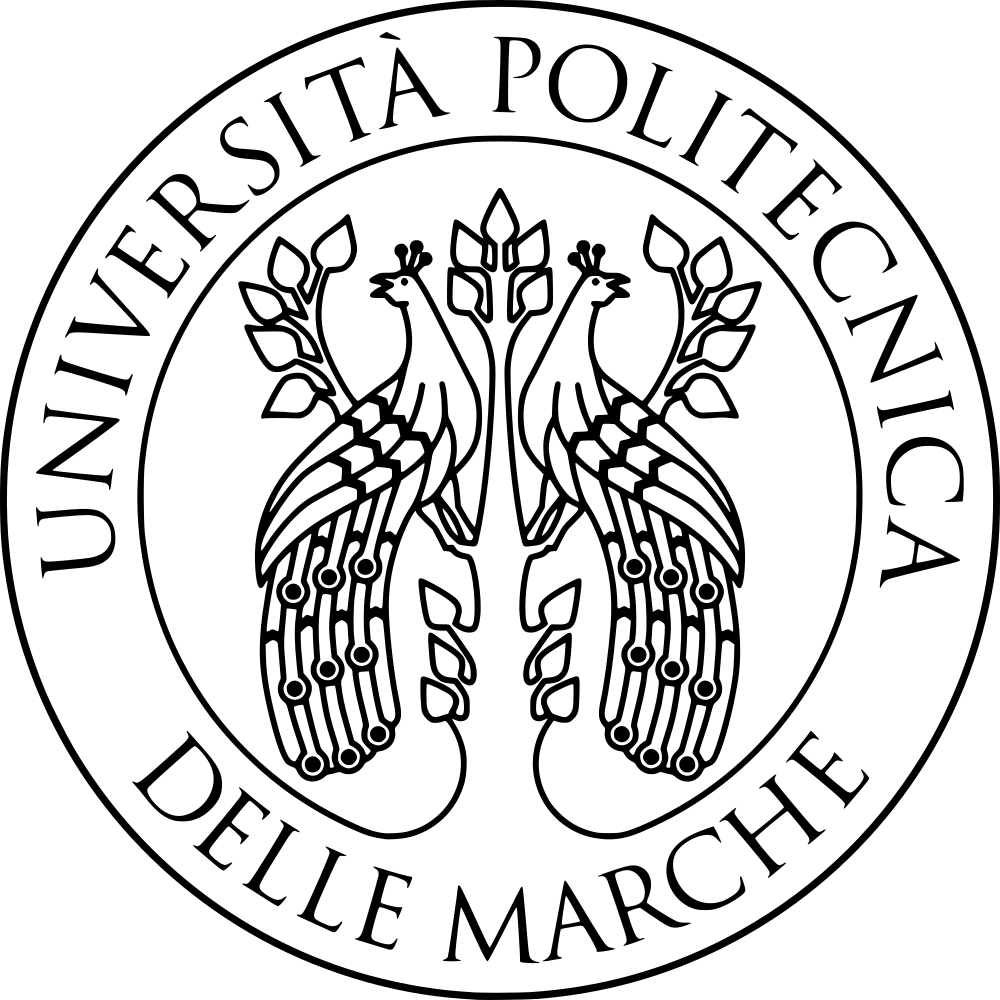
\includegraphics[width=3cm]{logo.png}
\end{figure}

\vspace{5mm}

\textbf{\color{black} \large \scshape Tesina di:}

\vspace{2mm}

\color{Green}\LARGE{\bf Business Intelligence}\color{black}
%accentColor
\vspace{4mm}

\large{Esame per il corso tenuto dal Prof. Domenico Ursino, durante l'anno accademico 2024-2025}

\vspace{4mm}

\large{9 CFU}

\vfill

\end{center} 	
\vspace{20mm} 	
\begin{center}
\flushleft{\small
% \emph{Questo documento è frutto di un'attenta sintesi tra materiale didattico fornito dal docente, spunti da lezioni e ulteriori approfondimenti. Il documento mira a offrire un quadro completo e dettagliato del corso, cercando di non tralasciare - salvo casi particolari - alcun dettaglio.}

\begin{dbBox}\small
Redazione del documento a cura di:
\begin{itemize}
    \item \textbf{\color{black}Chebbaki Anass} (Matr. 1124883) - \href{mailto:S1124883@studenti.univpm.it} {s1124883@studenti.univpm.it} 
    \item \textbf{\color{black}Sabatini Caterina} (Matr. 1121684) - \href{mailto:s1121684@studenti.univpm.it}{s1121684@studenti.univpm.it}
    \item \textbf{\color{black}Stronati Matteo} (Matr. 1122745) - \href{mailto:S1122745@studenti.univpm.it} {s1122745@studenti.univpm.it} 
\end{itemize}
\end{dbBox}\normalsize}

\centering


\rule{150mm}{.2mm}

\textbf{\color{black}\scshape Anno Accademico 2024-2025}\\
\textit{\scshape Anno I}
\end{center} 	


%----------------------------------------------------------------------------------------
%	TABLE OF CONTENTS
%----------------------------------------------------------------------------------------

%\usechapterimagefalse % If you don't want to include a chapter image, use this to toggle images off - it can be enabled later with \usechapterimagetrue

\chapterimage{tabl_cont3.pdf} % Table of contents heading image

\pagestyle{empty} % No headers

\tableofcontents % Print the table of contents itself

% \cleardoublepage % Forces the first chapter to start on an odd page so it's on the right

\pagestyle{fancy} % Print headers again

%----------------------------------------------------------------------------------------
%	PART
%----------------------------------------------------------------------------------------

%\part{Analisi del Dataset}

%----------------------------------------------------------------------------------------
%	CHAPTER 1
%----------------------------------------------------------------------------------------
\chapterimage{tabl_cont3.pdf} % Chapter heading image

\chapter{Introduzione}
Negli ultimi decenni, il cambiamento climatico è diventato uno dei temi centrali del dibattito scientifico e politico a livello globale. L'aumento delle temperature medie terrestri, il verificarsi di eventi meteorologici estremi e lo scioglimento dei ghiacciai rappresentano segnali inequivocabili di un fenomeno in continua evoluzione. Tra le principali cause di questo cambiamento, l'attività umana riveste un ruolo determinante, in particolare attraverso le emissioni di gas serra, come l'anidride carbonica (CO\textsubscript{2}), derivanti dalla produzione e dal consumo di energia.

Per condurre un'analisi approfondita su questo argomento, sono stati esaminati due dataset distinti: \textbf{FAOSTAT Temperature Change} e \textbf{Global Data on Sustainable Energy (2000-2020)}. Tali fonti di dati consentono di esplorare le dinamiche del cambiamento climatico e della transizione energetica, offrendo una visione complessiva e dettagliata delle tendenze globali nel corso del tempo.

\section{FAOSTAT Temperature Change}
Il primo dataset preso in considerazione per le analisi è stato \textbf{FAOSTAT Temperature Change}, il quale fornisce statistiche sulla variazione della temperatura superficiale media a livello nazionale, con aggiornamenti annuali. I dati coprono il periodo compreso tra il 1961 e il 2023 e riportano le anomalie della temperatura media mensile, stagionale e annuale, calcolate rispetto a una climatologia di riferimento corrispondente al periodo 1951-1980.

Le informazioni contenute nel dataset si basano sui dati \textit{GISTEMP}\footnote{I dati \textit{GISTEMP} (\textit{GISS Surface Temperature Analysis}) sono un set di dati sulla temperatura superficiale globale, sviluppato e mantenuto dalla NASA \textit{Goddard Institute for Space Studies} (\textit{GISS}). Questo dataset misura le anomalie della temperatura terrestre e oceanica, fornendo una panoramica dell'andamento del riscaldamento globale nel tempo.}, distribuiti pubblicamente dalla \textit{NASA-GISS} (\textit{National Aeronautics and Space Administration Goddard Institute for Space Studies}), e includono anche la deviazione standard della variazione di temperatura secondo la metodologia di base adottata. Tutte le variazioni di temperatura, presenti nei file \texttt{.csv}, sono calcolate su scala mensile, stagionale e annuale rispetto alla climatologia base del 1951-1980.

Dal punto di vista statistico, il dominio del cambiamento di temperatura segue le linee guida del \textit{Framework for the Development of Environmental Statistics} (\textit{FDES 2013}), contribuendo a fornire indicatori ambientali affidabili. L'unità statistica del dataset è costituita dai Paesi e Territori di tutto il mondo, con una copertura di 190 nazioni e 37 entità territoriali, secondo la classificazione \textit{FAOSTAT}\footnote{Il \textit{FAOSTAT} è un sistema di raccolta e diffusione dei dati statistici della \textit{Food and Agriculture Organization} (\textit{FAO}) delle Nazioni Unite. Fornisce un'ampia gamma di informazioni su agricoltura, alimentazione, risorse naturali e ambiente, coprendo oltre 245 paesi e territori, con serie temporali che spesso risalgono a diversi decenni.} e il livello amministrativo globale \textit{GAUL} della \textit{FAO}.

Il dataset offre un'importante risorsa per analisi climatiche dettagliate, consentendo lo studio delle variazioni di temperatura su scale temporali e geografiche diverse, contribuendo alla comprensione dei cambiamenti climatici a livello globale.
\newpage
Il dataset è composto da 4 file \texttt{.csv}:
\vspace{2mm}

\begin{itemize}
    \item\texttt{Environment\_Temperature\_Change\_E\_All\_Data\_NOFLAG.csv}: specifica i dati annuali sulle variazioni della temperatura superficiale media per paese dal 1961 al 2019.
    \item \texttt{FAOSTAT\_data\_1-10-2022.csv}: contiene i dati annuali sulle variazioni della temperatura superficiale media globale per paese, coprendo il periodo 1961-2020.
    \item \texttt{FAOSTAT\_data\_11-24-2020.csv}: contiene le definizioni e gli standard utilizzati in FAOSTAT.
    \item \texttt{FAOSTAT\_data\_11-1-2024.csv}: contiene i dati annuali sulle variazioni della temperatura superficiale media globale per paese, coprendo il periodo 1961-2023.
\end{itemize}
\vspace{2mm}
 Per le analisi presentate di seguito, è stato utilizzato esclusivamente il file \texttt{FAOSTAT\_data\_1-10-2022.csv}. Questa scelta metodologica è stata motivata dalla necessità di disporre di un dataset aggiornato, che raccoglie i dati più recenti fino all'anno 2020, analogamente al secondo dataset considerato. Tuttavia, il file selezionato è stato preferito in quanto offre misurazioni più precise e complete, garantendo una maggiore affidabilità nell'elaborazione statistica e nell'interpretazione dei risultati. Tale accuratezza ha consentito di condurre un'analisi approfondita e rigorosa, in linea con gli obiettivi dello studio.

 Nell'elenco \ref{elenco_dati1}, sono riportati i principali campi presenti file preso in esame:
\vspace{2mm}
\begin{enumerate}
\label{elenco_dati1}
    \item \texttt{Domain Code}: codice numerico che identifica il dominio di dati (es. agricoltura, emissioni, ecc.).
    \item \texttt{Domain}: nome del dominio dei dati.
    \item \texttt{Area Code (FAO)}: codice numerico assegnato dalla FAO ai paesi o regioni.
    \item \texttt{Area}: nome del paese o regione a cui si riferiscono i dati.
    \item \texttt{Element Code}: codice numerico che identifica la variabile misurata.
    \item \texttt{Element}: nome della variabile misurata.
    \item \texttt{Months Code}: codice numerico del mese (se applicabile).
    \item \texttt{Months}: nome del mese (se applicabile, altrimenti vuoto).
    \item \texttt{Year Code}: codice numerico dell'anno.
    \item \texttt{Year}: anno a cui si riferiscono i dati.
    \item \texttt{Unit}: unità di misura dei dati.
    \item \texttt{Value}: il valore effettivo della misura registrata.
    \item \texttt{Flag}: codice che indica una nota o una condizione particolare sui dati.
    \item \texttt{Flag Description}: descrizione testuale della nota.
\end{enumerate}



\section{Global Data on Sustainable Energy (2000-2020)}

Il dataset intitolato \textbf{Global Data on Sustainable Energy (2000-2020)}, rilasciato dall'autore Ansh Tanwar, fornisce una panoramica esaustiva e rigorosa degli indicatori energetici sostenibili su scala mondiale, coprendo un arco temporale di due decenni. Questa risorsa di elevato valore scientifico consente di analizzare in modo approfondito l'evoluzione dell'accesso all'elettricità, l'impiego delle energie rinnovabili, le emissioni di carbonio, l'intensità energetica, i flussi finanziari e la crescita economica di ciascun paese nel periodo compreso tra il 2000 e il 2020.

Attraverso un approccio comparativo, il dataset facilita il monitoraggio accurato dei progressi compiuti verso il conseguimento dell'\textit{Obiettivo di Sviluppo Sostenibile 7} (\textit{SDG 7}), il quale mira a garantire l'accesso universale a un'energia affidabile, sostenibile e moderna, a un costo economicamente sostenibile. L'analisi di tali dati consente non soltanto di individuare le tendenze globali e regionali, ma anche di identificare le aree in cui è necessario un impegno rafforzato per accelerare la transizione energetica.

Inoltre, il dataset rappresenta una solida base empirica per la costruzione di modelli predittivi, valutazioni di impatto ambientale e studi economici, rivelandosi pertanto uno strumento imprescindibile per ricercatori e professionisti operanti nel settore energetico.

Grazie alla sua ampiezza e profondità, questa raccolta di dati costituisce un'opportunità per approfondire la comprensione delle dinamiche energetiche globali e contribuire attivamente alla costruzione di un futuro più sostenibile e resiliente.

Il dataset è composto da un unico file denominato \texttt{global-data-on-sustainable-energy.csv}. Di seguito, nell'elenco \ref{elenco_dati2}, sono riportati i principali campi presenti all'interno del file:
\vspace{2mm}
\begin{enumerate}
\label{elenco_dati2}
    \item \texttt{Entity}: nome del paese o della regione per cui i dati sono riportati.
    \item \texttt{Year}: anno di riferimento dei dati, compreso tra il 2000 e il 2020.
    \item \texttt{Access to electricity (\% of population)}: percentuale della popolazione con accesso all'elettricità.
    \item \texttt{Access to clean fuels for cooking (\% of population)}: percentuale della popolazione che fa affidamento principalmente su combustibili puliti per cucinare.
    \item \texttt{Renewable-electricity-generating-capacity-per-capita}: capacità installata di energia rinnovabile per persona.
    \item \texttt{Financial flows to developing countries (US \$)}: flussi finanziari verso i paesi in via di sviluppo, sotto forma di aiuti e assistenza per progetti di energia pulita.
    \item \texttt{Renewable energy share in total final energy consumption (\%)}: percentuale di energia rinnovabile sul consumo finale totale di energia.
    \item \texttt{Electricity from fossil fuels (TWh)}: elettricità generata da combustibili fossili (carbone, petrolio, gas) espressa in terawattora.
    \item \texttt{Electricity from nuclear (TWh)}: elettricità prodotta da energia nucleare, in terawattora.
    \item \texttt{Electricity from renewables (TWh)}: elettricità generata da fonti rinnovabili (idroelettrica, solare, eolica, ecc.) in terawattora.
    \item \texttt{Low-carbon electricity (\% electricity)}: percentuale di elettricità prodotta da fonti a basse emissioni di carbonio (nucleare e rinnovabili).
    \item \texttt{Primary energy consumption per capita (kWh/person)}: consumo di energia primaria per persona, espresso in kilowattora.
    \item \texttt{Energy intensity level of primary energy (MJ/\$2011 PPP GDP)}: livello di intensità energetica dell'energia primaria, misurato in megajoule per unità di PIL a parità di potere d'acquisto (PPP) del 2011.
    \item \texttt{Value\_co2\_emissions (metric tons per capita)}: emissioni di anidride carbonica per persona, espresse in tonnellate metriche.
    \item \texttt{Renewables (\% equivalent primary energy)}: percentuale dell'energia primaria equivalente derivante da fonti rinnovabili.
    \item \texttt{GDP growth (annual \%)}: tasso di crescita annuale del GDP, basato sulla valuta locale costante.
    \item \texttt{GDP per capita}: prodotto interno lordo per persona.
    \item \texttt{Density (P/Km2)}: densità di popolazione, espressa in persone per chilometro quadrato.
    \item \texttt{Land Area (Km2)}: superficie totale del territorio, espressa in chilometri quadrati.
    \item \texttt{Latitude}: latitudine del centroide del paese, in gradi decimali.
    \item \texttt{Longitude}: longitudine del centroide del paese, in gradi decimali.
\end{enumerate}

%PREPPROCESSING DEL DATASET?
%----------------------------------------------------------------------------------------

%	CHAPTER 2
%----------------------------------------------------------------------------------------
\chapterimage{tabl_cont3.pdf} % Chapter heading image

\chapter{Qlik}
\section{Introduzione}
\textbf{Qlik} è una società statunitense di software, con sede in Pennsylvania, fondata nel 1993 a Lund, in Svezia. La compagnia, il cui logo è mostrato alla Figura \ref{fig:QlikLogo}, è nota per aver sviluppato una piattaforma avanzata di Business Intelligence, che consente alle aziende di trasformare i propri dati in informazioni strategiche attraverso tecniche di analisi visiva e interattiva. Utilizzando il motore associativo, Qlik permette agli utenti di esplorare i dati in modo dinamico, creando visualizzazioni intuitive volte a semplifiicare il processo decisionale. La capacità di integrare e visualizzare grandi volumi di dati provenienti da diverse fonti in tempo reale rappresenta uno degli aspetti distintivi della piattaforma, rendendo Qlik uno strumento potente per analisi complesse e reporting.

\begin{figure}[h!]
    \centering
    
\includegraphics[width=0.35\linewidth]{capitolo_1/img1/QlikLogo.pdf}
    \caption{Qlik - Logo}
    \label{fig:QlikLogo}
\end{figure}

Qlik offre diverse applicazioni e strumenti, tra cui Qlik Sense e QlikView, che rispondono a diverse esigenze di business e di analisi dei dati. \textbf{Qlik Sense} è una piattaforma di Business Intelligence self-service progettata per offrire una creazione di report e dashboard personalizzati, con una forte enfasi sull'interattività e sulla visualizzazione dei dati. Grazie alla sua interfaccia intuitiva, Qlik Sense consente agli utenti di esplorare i dati autonomamente, creando visualizzazioni dinamiche e analisi ad hoc senza necessitare di competenze tecniche avanzate. Inoltre, Qlik Sense si distingue per la sua capacità di adattarsi facilmente a diverse fonti di dati, offrendo funzionalità di drag-and-drop, capacità di collaborazione e scalabilità in ambienti aziendali complessi. È particolarmente adatto a organizzazioni che desiderano democratizzare l'accesso ai dati, dando a tutti i livelli aziendali la possibilità di fare analisi e prendere decisioni basate sui dati in tempo reale.

D'altra parte, \textbf{QlikView} è una soluzione di BI più tradizionale e predefinita, progettata per rispondere a esigenze aziendali strutturate e complesse. Mentre Qlik Sense è più orientato all’autonomia dell'utente, QlikView richiede una configurazione più tecnica e un'implementazione più centralizzata. È ideale per le aziende che necessitano di soluzioni di reporting più fisse e predeterminate, dove l'analisi è spesso guidata da requisiti specifici di business e processi consolidati. QlikView consente la creazione di applicazioni di analisi altamente personalizzate e report standardizzati, spesso progettati da sviluppatori IT o team di BI, per soddisfare le necessità analitiche in modo scalabile e sicuro.

La versatilità della piattaforma consente di rispondere in modo rapido alle necessità aziendali, migliorando la capacità di prendere decisioni informate e basate su dati concreti. In tale contesto, l'adozione di Qlik consente alle organizzazioni di ottimizzare i propri processi aziendali, ottenere insight più approfonditi e supportare strategie orientate alla crescita.


\subsection{Caricamento e preparazione del dataset}
Il processo di caricamento dei dati su Qlik è una fase cruciale che consente di importare e integrare dati provenienti da diverse fonti e in vari formati, tra cui database relazionali come \textit{SQL Server}, \textit{Oracle} e \textit{MySQL}, file flat (\textit{CSV}, \textit{Excel}), applicazioni cloud come \textit{Google Analytics} e \textit{Salesforce}, nonché altre fonti esterne.
A differenza di altri strumenti di Business Intelligence, Qlik Sense mette a disposizione un \textbf{Associative Engine}\footnote{Contrariamente a Qlik, la maggior parte degli strumenti di Business Intelligence odierni si fonda su database relazionali e adotta un approccio basato su query, il che può risultare limitante. Infatti, SQL non è stato progettato per supportare analisi interattive dei dati, restringendo così le opportunità di esplorazione dinamica.}. Quest'ultimo è una componente fondamentale che consente di eseguire calcoli e aggregazioni in tempo reale, senza necessità di attendere operazioni di aggiornamento da parte dello sviluppatore. Questo motore permette di aggiornare le analisi dinamicamente, facilitando l'esplorazione dei dati e mettendo in evidenza le relazioni tra diverse informazioni. Grazie a questa capacità di calcolo «on-the-fly», gli utenti possono interagire con i dati in modo immediato, senza dover aspettare una risposta statica predefinita. Questo elimina il tradizionale ciclo di lavoro «ask, wait, answer», dove gli utenti erano costretti a fare una domanda, attendere che venisse sviluppata una risposta e infine ricevere l'informazione desiderata. Con Qlik, invece, l'analisi è continua e interattiva, consentendo un'esplorazione autonoma e in tempo reale dei dati, il che migliora notevolmente l'efficienza decisionale e la reattività alle domande aziendali.

Per le analisi proposte in seguito, sono stati caricati i file \texttt{FAOSTAT\_data\_1-10-2022.csv}, configurando le impostazioni necessarie ad una corretta lettura del dataset, come la selezione del tipo di delimitatore. Per una corretta gestione dei dati, è stata utilizzata la sezione \textit{Editor di Script}, per modificare parte dei campi tramite codice.

La modifica più rilevante ha riguardato l'ordine dei mesi inseriti nel campo \texttt{Months}, che si presentavano in una sequenza sbagliata rispetto a quella canonica. Innanzitutto, sono stati mappati i mesi in numeri mediante il Codice \ref{codice_mesi}, proposto in seguito. In questo modo è stata creata una nuova colonna \texttt{MonthNum}, che contiene i numeri associati ai mesi.
\newpage
\begin{lstlisting}[language=Qlik, caption={Mapping dei mesi}, captionpos=b]
MonthMap:
LOAD * INLINE [
    Month, MonthNum
    'January', 1
    'February', 2
    'March', 3
    'April', 4
    'May', 5
    'June', 6
    'July', 7
    'August', 8
    'September', 9
    'October', 10
    'November', 11
    'December', 12
];
\end{lstlisting}
\label{codice_mesi}

Successivamente, tramite la funzione \texttt{ApplyMap}, sono stati ricostruiti i riferimenti nominali, così da far apparire i nomi sui grafici.
In seguito, è presentato il Codice \ref{codice_load} di \texttt{LOAD} del dataset, in cui va notata il cambio di tipo associato al campo \texttt{Year} e \texttt{Value}.

\begin{lstlisting}[language=Qlik, caption={Caricamento dati FAOSTAT in Qlik}, captionpos=b]
 [FAOSTAT_data_1-10-2022]:
LOAD
    [@3] AS [Area_Code(FAO)],
    [@4] AS [Area],
    [@7] AS [Months_Code],
    ApplyMap('MonthMap', [@8], 0) AS MonthNum,
    [@9] AS [Year_Code],
    Date(Date#([@10], 'YYYY') ,'YYYY') AS [Year],
    Num(Replace([@12], ',', '.'), '#,##0.000') AS [Value],
    [@14] AS [Flag],
    ApplyMap('__countryCodeIsoThree2Polygon', 
    ApplyMap('__countryName2IsoThree', LOWER([@4])), '-') AS [FAOSTAT_data_1-10-2022.@4_GeoInfo]
FROM [lib://DataFiles/FAOSTAT_data_1-10-2022.csv]
(txt, utf8, no labels, delimiter is ',', msq, header is 1 lines);
 
\end{lstlisting}
\label{codice_load}

Una volta eseguito lo script, Qlik carica i dati, creando un modello associativo che
facilita l'analisi interattiva.

\section{Data Analysis Dataset FAOSTAT Temperature Change}

Dopo aver caricato i dati, sono state create delle \textbf{Dashboard} con l'obiettivo di analizzare il dataset in modo approfondito. Questi strumenti consentono un'analisi dettagliata grazie a diverse funzionalità, tra cui grafici e filtri applicabili per affinare l'esplorazione dei dati.  

L'analisi è stata condotta utilizzando Qlik, focalizzandosi sul dataset \textbf{FAOSTAT Temperature Change}. Di seguito, vengono presentate le dashboard impiegate per le prime fasi dell'analisi:

\begin{itemize}
    \item \textbf{Analisi della variazione della Temperatura Media};
    \item \textbf{Visualizzazione geospaziale della variazione della Temperatura Media nel mondo};
\end{itemize}

\section{Analisi della variazione della Temperatura Media}
La Dashboard mostrata in Figura \ref{fig:dashboard_world} analizza la variazione del valore della temperatura media nel mondo, tra il 1961 e il 2020. 

\begin{figure}[h!]
    \centering
    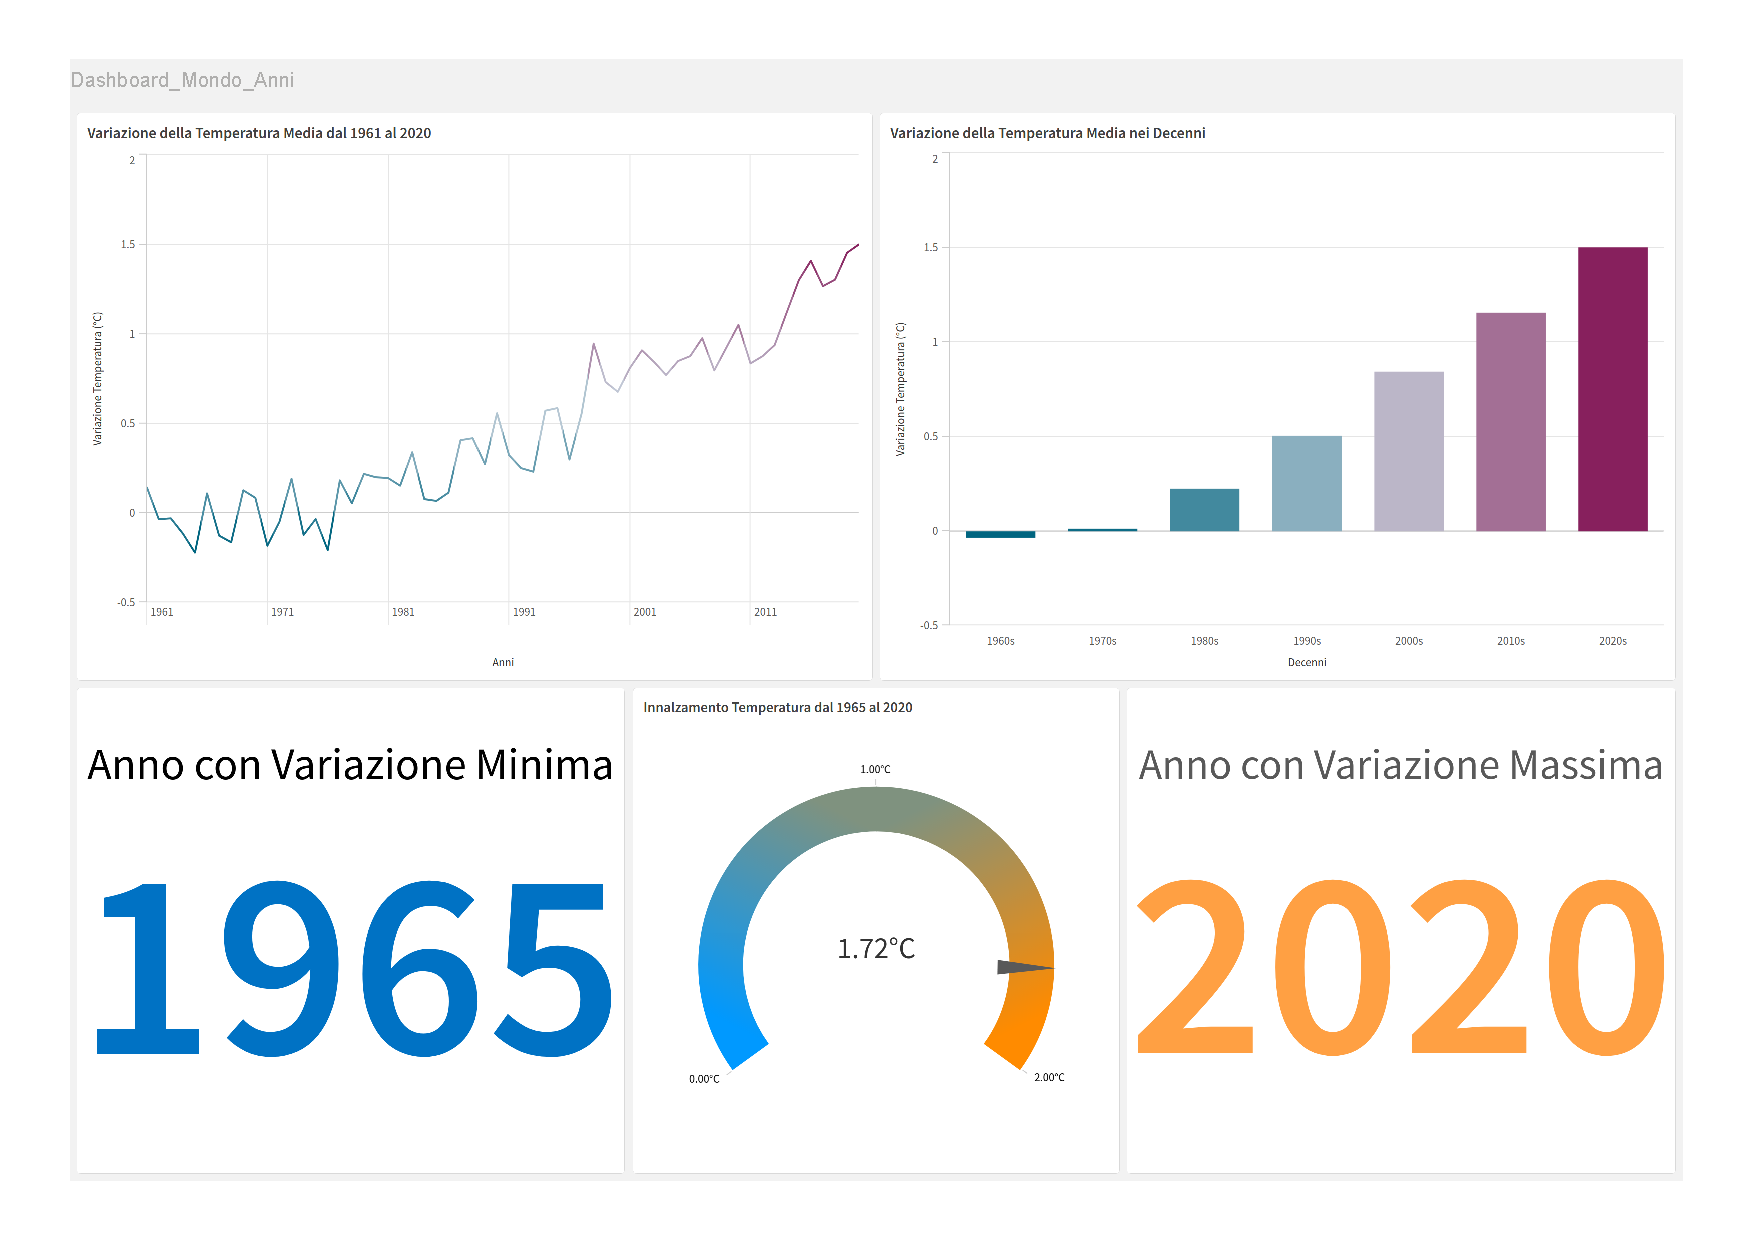
\includegraphics[width=1\linewidth]{capitolo_2/img2/Dashboard_world.pdf}
    \caption{Analisi della variazione della Temperatura Media}
    \label{fig:dashboard_world}
\end{figure}

\subsection{Struttura Dashboard}

\subsection{Filtri applicati}

\begin{comment}
    FARE PROCESSAMENTO DEL DATASET -> UNIONE DATASET
\end{comment}
%----------------------------------------------------------------------------------------
%	CHAPTER 3
%----------------------------------------------------------------------------------------
\chapterimage{tabl_cont3.pdf} % Chapter heading image

\chapter{Tableau}

%----------------------------------------------------------------------------------------
%	CHAPTER 4
%----------------------------------------------------------------------------------------
\chapterimage{tabl_cont3.pdf} % Chapter heading image

\chapter{PowerBI}
%----------------------------------------------------------------------------------------

%	BIBLIOGRAPHY
%----------------------------------------------------------------------------------------

 %\chapter*{Bibliography}
 %\addcontentsline{toc}{chapter}{\textcolor{Green}{Bibliography}}
 %\section*{Books}
 %\addcontentsline{toc}{section}{Books}
 %\printbibliography[heading=bibempty,type=book]
 %\section*{Articles}
 %\addcontentsline{toc}{section}{Articles}
 %\printbibliography[heading=bibempty,type=article]

% %----------------------------------------------------------------------------------------
% %	INDEX
% %----------------------------------------------------------------------------------------

% \cleardoublepage
% \phantomsection
% \setlength{\columnsep}{0.75cm}
% \addcontentsline{toc}{chapter}{\textcolor{Green}{Index}}
% \printindex


%----------------------------------------------------------------------------------------

\end{document}
